\chapter{Implementation}
\label{chap:implementation}

\begin{introduction}

Building upon the conceptual architecture proposed in Chapter~\ref{chap:proposed_solution}, this chapter delves into the practical implementation of the Resilient Federated Learning Framework. It details the technical choices made and the components developed to realize a modular and resilient system capable of operating in dynamic network environments. The following sections describe the selected software stack, the implementation details of the \ac{fl} algorithms, including specific resilience mechanisms and optimizations, additional features built to support the framework, and key technical considerations such as communication protocol specifics, worker scheduling, and framework extensibility.

\end{introduction}


\section{Software Stack}
\label{sec:technology-stack}

Figure~\ref{fig:technology-stack} provides an overview of the software stack used in implementing the Resilient Federated Learning Framework. The diagram illustrates the various components and their interactions, highlighting the system's modularity and flexibility.

\begin{figure}[!htbp]
    \centering
    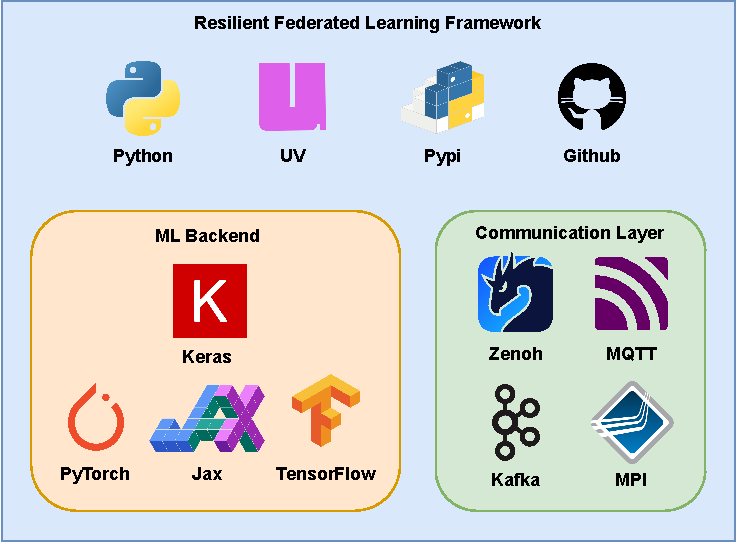
\includegraphics[width=0.8\textwidth]{figs/technology-stack.pdf}
    \caption[Software Stack of the Resilient FL Framework]{Diagram presenting the key software components comprising the Resilient \ac{fl} Framework, including core development tools, interchangeable \ac{ml} backends, and diverse communication protocols, emphasizing its modular design.}
    \label{fig:technology-stack}
\end{figure}

The implementation of the proposed framework is built primarily using Python. This choice was motivated by Python's widespread adoption and robust ecosystem within the data science and \ac{ml} communities, offering a balance of ease of use and performance through highly optimized libraries, as highlighted by \citeauthor{raschka2020machine} in their survey of the field \cite{raschka2020machine}.

For effective management of project dependencies and ensuring reproducible development environments, crucial for any substantial software project, we used UV~\footnote{\url{https://docs.astral.sh/uv/}}. UV is an extremely fast Python package and project manager, written in Rust. It is known for its significant speed advantages over traditional tools like pip and aims to consolidate the functionality of multiple tools (such as pip, pip-tools, and virtualenv) into a single, efficient utility. UV provides comprehensive features including dependency resolution, package installation, virtual environment creation, and even Python version management, making it a powerful choice for streamlining the development workflow. 

Version control is indispensable for tracking changes, collaborating, and maintaining a software project's history. Git was employed for this purpose, with the framework's codebase hosted on GitHub~\footnote{\url{https://github.com/leoalmPT/FlexFL}}. The choice of GitHub aligns with industry standards and best practices for software development, ensuring that the project is accessible to contributors and users alike. The publicly available repository allows for transparency and community engagement in the development process.

The implemented framework is available as a standard Python package on the \ac{pypi} to facilitate easy access and distribution for other researchers and practitioners. This availability allows users to effortlessly install the framework and its dependencies using simple commands (e.g., \texttt{pip install flexfl}), providing both a Python library for programmatic use and a \ac{cli} tool for direct execution and experimentation, contributing to the goal of making the framework an open-source resource.

For the core \ac{ml} operations, the framework needed to integrate with established \ac{ml} libraries. While several powerful libraries exist, TensorFlow, PyTorch, and JAX are currently among the most widely used in the Python ecosystem for deep learning and numerical computation. These libraries, however, differ significantly in their \acp{api}, design philosophies, and typical use cases. As mentioned in Chapter~\ref{chap:proposed_solution}, the ML Backend module of our framework is designed specifically to abstract away these differences, providing a consistent interface for the rest of the system regardless of the underlying \ac{ml} library. 

In this implementation, we have built support primarily around Keras, a high-level \ac{api} that acts as a powerful abstraction layer. The Keras philosophy emphasizes that it is a deep learning \ac{api} designed with a focus on debugging speed, code elegance and conciseness, maintainability, and deployability. Crucially, Keras achieves this while offering a multi-backend approach, giving users the freedom to work with JAX, TensorFlow, and PyTorch, and allowing them to build models that can move seamlessly across these frameworks and leverage the strengths of each ecosystem. Additionally, we have also integrated support for TensorFlow and PyTorch directly, allowing users to choose the backend that best fits their needs. This flexibility is essential for researchers and practitioners who may have specific requirements or preferences for their \ac{ml} workflows.

Moving to the communication infrastructure, a critical component for coordinating clients and the server in a distributed setting, we implemented support for all four protocols discussed in Chapter~\ref{chap:background}: \ac{mpi} (via Open \ac{mpi}), \ac{mqtt}, Kafka, and Zenoh. While \ac{mpi} may not be ideally suited for the dynamic network environments inherent in \ac{fl} due to its reliance on static configurations and lack of built-in fault tolerance for node failures, its inclusion serves as a valuable benchmark for performance comparison, given its prevalence and optimization for speed in \ac{hpc} environments. 

The implementation of \ac{mqtt}, Kafka, and Zenoh, on the other hand, allows the framework to leverage protocols better designed for dynamic and potentially unreliable networks, offering flexibility and enabling empirical evaluation of their performance and the framework's resilience mechanisms under conditions with and without worker failures or disconnections.



\section{Federated Learning Algorithms}
\label{sec:federated-learning-algorithms}

Building upon the architectural principles established in Chapter~\ref{chap:proposed_solution} and the algorithmic taxonomy discussed in Chapter~\ref{chap:background}, our framework implements the four primary types of \ac{fl} algorithms to demonstrate versatility and evaluate performance across different collaboration and scheduling paradigms. These are Centralized Synchronous, Centralized Asynchronous, Decentralized Synchronous, and Decentralized Asynchronous algorithms. Each algorithm is designed to operate within the framework's modular architecture, allowing for easy integration and experimentation with various components.

These standard algorithmic implementations incorporate several key adaptations and features beyond their basic theoretical descriptions to address the objectives of resilience and modularity in dynamic network environments. These are discussed in detail in this section.

\subsection{Dynamic Worker Pool and Epoch Definition}
\label{sec:dynamic-worker-pool}

A core adaptation, facilitated by the Worker Manager module, is managing a dynamic pool of potential workers. Instead of assuming a fixed set of participating devices, the framework dynamically selects a \texttt{subpool} of available and suitable workers at the start of each training round or epoch. This allows devices to join or leave the network seamlessly without disrupting the training process, contributing directly to elasticity and resilience.

Within our framework, a training \texttt{epoch} or \texttt{round} represents a complete cycle of global model coordination and update involving the selected worker subpool. A key parameter governing this process is the concept of \texttt{iterations} per epoch for Synchronous approaches. This defines the number of times that the parameter server sends tasks to the workers and collects their updates. The definition of epochs and iterations depends on the algorithm type:

\begin{itemize}
    \item \textbf{Centralized Approaches:} The primary task for each worker in a round is to receive the current global model, compute gradients on a local mini-batch, and send these gradients to the Parameter Server. The total number of effective computations (tasks) in a round is thus related to the sum of the number of batches processed by all selected workers. The number of iterations is defined by the total number of tasks divided by the number of workers in the subpool. 
    \item \textbf{Decentralized Approaches:} Each worker's task in a round involves performing a specified number of local epochs and then exchanging their resulting local model or parameters with the parameter server. One global synchronization round corresponds to each selected worker completing their local training phase and submitting their updates. Only 1 iteration is performed per round.
\end{itemize}

\subsection{Resilience Mechanisms}
\label{sec:resilience-mechanisms}

Regardless of the algorithm type, the framework implements resilience mechanisms to handle worker failures and disconnections. These mechanisms are designed to ensure that the training process can continue despite unexpected disruptions, aligning with the framework's goal of resilience in dynamic network environments.

In Asynchronous algorithms, where the system can tolerate some delays, the framework monitors the progress of tasks assigned to workers in the worker subpool. If a worker fails, disconnects, or becomes unresponsive while executing its task (either gradient computation in centralized async or local training in decentralized async), the Worker Manager detects it. 

The task associated with the failed worker can then be automatically rescheduled and assigned to another available worker from the dynamic pool, according to the scheduling policy, ensuring that the necessary contribution for the round is eventually completed. If the number of workers drops below a certain threshold, the Parameter Server will pause the training round by stopping the distribution of new tasks until the Worker Manager detects that enough workers are available again.   

Synchronous algorithms inherently require a higher degree of coordination. To prevent single stragglers or failures from halting the entire training process, a configurable completion threshold (e.g., 50\%) is introduced for each iteration. If the number of workers in the selected worker subpool that successfully complete and submit their tasks meets or exceeds this threshold, the Parameter Server proceeds with the aggregation step using the available updates. This allows the training to advance even if a subset of workers fails or is significantly delayed.

\subsection{Optimizations}
\label{sec:optimizations}

Several optimizations have been incorporated into the framework to enhance its efficiency and scalability, particularly in handling large models and coordinating multiple workers.

A key optimization concerns aggregating model weights or gradients received from workers on the Parameter Server. To conserve memory and avoid the need to store the whole model or gradient updates from every worker simultaneously, the aggregation process is performed on the fly. As updates arrive from individual workers, they are incrementally incorporated into a running weighted sum or average. This allows the memory associated with a worker's update to be released immediately after it has been processed. 

For instance, if $M$ represents the size of a single model update and there are $N$ workers, this approach reduces the server's peak memory footprint from potentially $N \times M$ bytes (if all updates were buffered simultaneously) to approximately $2 \times M$ bytes (for the current global model and one incoming update). This significantly enables support for a larger number of workers or larger model sizes than would otherwise be possible.

Furthermore, to minimize idle time and increase overall throughput, the framework optimizes the timing of task distribution to workers. Instead of waiting for the Parameter Server to complete the full validation process on the newly updated global model, tasks for the next round can be initiated as soon as the global model state is mathematically finalized by the aggregation process. This helps to pipeline the training process, reducing the latency between rounds. 

For example, if validation for each epoch takes $T$ seconds and the training runs for $E$ epochs, this optimization can reduce the total training time by up to $E \times T$ seconds by overlapping validation with the start of the subsequent round, thereby improving the utilization of both the server and worker resources, especially when the Parameter Server is not a bottleneck.

Additionally, a crucial change for asynchronous approaches was made. With dynamic worker participation, we must ensure that workers train on models that do not excessively lag behind the global model. In the original decentralized asynchronous algorithms, model differences were used for updates, but this is not suitable when workers might skip rounds due to the dynamic pool selection. To address this, at the start of each round, the Parameter Server sends the current global model to all workers in the current subpool, and each worker then performs their tasks using this model. This ensures that, despite the asynchronous nature and potential for variable participation, workers start their local computations from a recent common reference point, which helps convergence stability.



\section{Additional Features}
\label{sec:additional-features}

Beyond the core modular architecture and implemented \ac{fl} algorithms, the framework provides a suite of additional features, primarily exposed through \ac{cli} tools. These tools are designed to streamline the entire Federated Learning workflow, from data preparation and setup to experimentation, simulation, and analysis, making the framework more accessible and practical for researchers and practitioners. 

The primary \ac{cli} commands available are:

\begin{itemize}
    \item \texttt{flexfl}: This is the main command for executing \ac{fl} experiments. It provides extensive configuration options through command-line arguments to define the setup of all seven core modules of the framework, enabling flexible experimentation with different algorithm types, communication protocols, ML backends, datasets, and more. Details on the argument parser and configuration options will be provided later in Section~\ref{sec:technical-details}.
    \item \texttt{flexfl-preprocess}: Used to manage the dataset preparation process. This command facilitates the downloading and initial preprocessing of datasets, allowing users to prepare data for specific experiments or batch-process multiple datasets supported by the framework's Dataset Manager module.
    \item \texttt{flexfl-division}: Handles the division of datasets for distributed training. This command splits processed datasets into training, validation, and testing sets. Crucially for \ac{fl}, it also partitions the training data among a specified number of workers, supporting both \ac{iid} and \ac{non-iid} data distributions to simulate various real-world scenarios encountered in \ac{fl}.
    \item \texttt{flexfl-benchmark}: Provides tools for benchmarking communication performance and resilience of the network layer. Designed to be run typically on two nodes (one acting as a server, one as a worker), this command allows for testing specific communication protocols implemented in the Communication Layer, simulating basic worker failures, and measuring the time required to send and receive payloads of varying sizes multiple times between nodes.
    \item \texttt{flexfl-res}: A utility specifically for simulating worker resilience under failure conditions. This command launches a specified process (e.g., a worker instance) and introduces controlled disruptions by randomly killing and restarting the process based on configurable probabilities and time intervals. This tool is helpful for empirically testing the fault tolerance mechanisms integrated into the framework under realistic failure scenarios.
    \item \texttt{flexfl-plot}: Dedicated to visualizing experiment results and system performance, this command processes the structured logs generated by framework runs and automatically generates various data visualizations, including plots and tables, for analyzing key metrics such as communication times, worker computation times, worker timelines, size of exchanged payloads, and overall run duration. This aids in understanding performance characteristics and the impact of different configurations.
\end{itemize}

These \ac{cli} tools collectively provide a comprehensive environment for setting up, running, simulating, and analyzing \ac{fl} experiments with the proposed framework, facilitating both research and practical application. But while these tools provide the interface for configuring and running \ac{fl} experiments on individual nodes, conducting realistic distributed and \ac{fl} studies requires managing a cluster of interconnected machines. 

To address the complexities of creating, configuring, and managing a fleet of \acp{vm} for experimentation, a separate package named \texttt{pxm-tools} and also available on \ac{pypi} was created. This tool leverages the Proxmox Virtual Environment \ac{api}, a widely used open-source platform for virtualization management. \texttt{pxm-tools} provides a command-line interface designed for ease of use when performing bulk operations on \acp{vm}. 

Its core functionalities include easily creating, editing, removing, starting, and stopping multiple \acp{vm} simultaneously. It also offers flexible configuration by allowing any argument available through the Proxmox \ac{api} to be set during \ac{vm} creation or editing. This is crucial for simulating diverse and heterogeneous environments by configuring \ac{vm} resources like the number of CPU cores, RAM size, storage, and critically, network interface bandwidth limits. The ability to control network conditions is essential for evaluating the framework's resilience under varying real-world constraints. 

Furthermore, \texttt{pxm-tools} automatically retrieves necessary \ac{vm} information, such as their unique IDs and assigned IP addresses, which are vital for subsequent interaction and logging. By abstracting the direct interaction with the Proxmox \ac{api} into simple \ac{cli} commands, \texttt{pxm-tools} significantly simplifies the process of setting up and tearing down experimental clusters, enabling rapid iteration and evaluation cycles.

Once the experimental \acp{vm} are provisioned and configured using \texttt{pxm-tools}, an efficient method is needed to interact with all or a subset of these machines collectively. Custom scripts were developed to enable parallel execution of commands across the chosen \acp{vm}, leveraging \ac{ssh} for secure communication. 

These scripts are designed to streamline the experimental workflow by allowing users to execute arbitrary shell commands concurrently on all selected \acp{vm}, drastically reducing the time required for setup tasks like installing dependencies or configuring the environment. They also efficiently distribute the preprocessed and partitioned datasets (prepared using \texttt{flexfl-division}) to the corresponding worker \acp{vm}, ensuring each node receives its designated data split for the experiment, and gather experimental outputs, such as logs, performance metrics, and final models, from all participating \acp{vm} in parallel after a run is complete. 

Finally, these scripts can launch the main \texttt{flexfl} command on the designated server \ac{vm} and all selected worker \acp{vm} simultaneously to initiate a distributed training run. These parallel interaction scripts, combined with \texttt{pxm-tools}, provide a complete toolchain for managing the experimental environment and executing Federated Learning experiments at scale on a cluster of \acp{vm}, crucial for thoroughly evaluating the framework's performance and resilience.



\section{Technical Details}
\label{sec:technical-details}

This section delves into the technical intricacies of the framework's implementation, focusing on key aspects such as the communication layer protocols, the worker scheduling policy, the functionality of the Worker Manager, early stopping mechanisms, the configuration interface via the argument parser and optional libraries, how experimental results are saved, and guidelines for extending the framework. These details highlight the practical realization of the modular and resilient design principles discussed in Chapter~\ref{chap:proposed_solution}.

\subsection{Communication Protocols}
\label{sec:comm-protocols-caveats}

As discussed in Chapter~\ref{chap:background}, the framework implements support for multiple communication protocols (Zenoh, \ac{mqtt}, Kafka, and \ac{mpi}) to offer flexibility and adaptability to diverse network environments. While the Communication Layer module provides a consistent \texttt{send} and \texttt{recv} interface to the rest of the framework, there are protocol-specific nuances and implementation details, particularly regarding asynchronous operation and fault detection.

All supported protocols require an initial connection phase where workers register with the Parameter Server to obtain a unique identifier and establish communication channels. The implementations for Zenoh and  \ac{mqtt} leverage their native support for asynchronous message handling, typically through threading or event loops, and include built-in capabilities to detect client disconnections (e.g., via callbacks or subscription mechanisms). This native support simplifies the implementation of resilience features dependent on knowing worker connection status.

Kafka, in contrast, is optimized for high-throughput, persistent message streaming and lacks native real-time disconnection notifications without incurring significant partition rebalancing overhead, which is undesirable in a dynamic \ac{fl} setting. To overcome this, the Kafka implementation required a manual heartbeat mechanism, where workers periodically send health check messages to the server. 

\ac{mpi}, being primarily designed for synchronous, blocking communication in high-performance computing environments, inherently operates in a request-response manner. But, as previously mentioned, it lacks built-in capabilities to detect client disconnections directly at the protocol level without explicit application-level checks, which imposes constraints on handling dynamic worker pools compared to the other protocols.

\subsection{Worker Scheduling Policy}
\label{sec:worker-scheduling-policy}

The framework incorporates a worker scheduling policy that is responsible for selecting the subset of available workers participating in each training round or epoch. The currently implemented policy is Round Robin, a well-established \cite{rasmussen2008round}, simple, and fair scheduling approach that cycles through the pool of available workers. In our dynamic setting, the Round Robin scheduler selects workers sequentially from the currently connected pool at the start of each round.

A key advantage of the framework's modular design is that the scheduling policy is encapsulated within the \ac{fl} algorithm. This allows users to easily replace the default Round Robin implementation with alternative policies (e.g., based on worker capabilities, data distribution, historical performance, or network conditions) to suit specific requirements, without needing to modify other core components of the framework. The scheduler's integration with the dynamic worker pool management enables seamless adaptation to workers joining or leaving the training process.

\subsection{Worker Manager}
\label{sec:worker-manager}

The Worker Manager is a pivotal module for achieving resilience and abstracting the complexities of dynamic worker participation from the core \ac{fl} algorithms. It acts as the central coordinator on the Parameter Server and also runs a client-side component on each worker. Its core functionalities include managing the list of currently connected workers and the selection of the worker subpool for each round, effectively hiding the complexities of workers joining or leaving from the \ac{fl} algorithm logic. 

Users can configure custom callbacks for key events, such as when a new worker joins the system (executable on both the Parameter Server and the joining worker) or  when a worker disconnects or fails (primarily handled on the Parameter Server). These callbacks allow for custom logic to be executed during these events, enhancing flexibility.

Communication within the framework is structured using message types (e.g., work, work\_done). that the user specifies when sending messages. The Worker Manager facilitates flexible message reception by allowing users to register callbacks to be executed automatically when a message of a specific type is received, which enables asynchronous processing of incoming messages. 

Users can also perform blocking receives for messages of a specific type, waiting until a message of that type arrives. Furthermore, the framework allows for the combination of blocking receives with callbacks. During a blocking wait for a specific message type, the Worker Manager can process other incoming messages in the background using their registered callbacks, such as join messages.

Integrated with the message handling, the Worker Manager monitors blocking receive operations for worker failure detection and rescheduling. If a worker fails or disconnects while a blocking receive is pending for a task assigned to it, the Worker Manager can trigger a user-defined callback that allows for the implementation of task rescheduling logic, enabling the framework to assign the failed task to another worker.

Messages received in the background that do not have an immediate callback registered are stored in an internal queue, so blocking receive operations first check this queue before waiting for new messages from the communication layer, ensuring that already received messages are processed promptly. The manager can also store relevant metadata for each connected worker, regarding the \ac{fl} training or potentially performance metrics, which can be used by scheduling policies or custom callbacks.

Finally, the Worker Manager provides a mechanism for conditional waiting, allowing the process to wait for a specific condition (defined by a callback function) to become true while the manager continues to process incoming messages in the background. This is useful for coordinating actions that depend on the state of multiple workers or received messages.

Figure~\ref{fig:worker-manager} presents a detailed flow diagram that illustrates how incoming messages are processed, how callbacks enable asynchronous handling and how the internal queue manages background messages, underscoring the robust communication pipeline designed to support the framework's operations under challenging conditions.

\begin{figure}[!htbp]
    \centering
    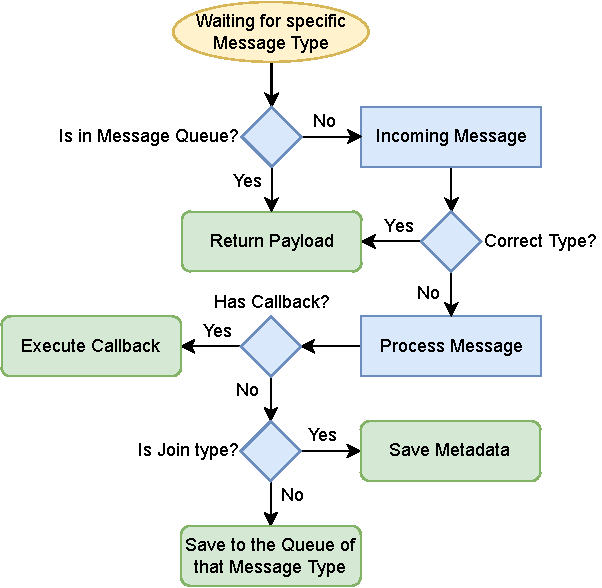
\includegraphics[width=0.7\textwidth]{figs/worker-manager.pdf}
    \caption[Worker Manager Message Processing Flow]{Flow diagram illustrating the Worker Manager's message processing, callback handling, and internal queue management.}
    \label{fig:worker-manager}
\end{figure}

\subsection{Early Stopping}
\label{sec:early-stopping}

To prevent overfitting and optimize training time, the framework implements an early stopping mechanism controlled on the Parameter Server. This feature allows users to define criteria for halting the training process based on the model's performance on a validation set. Configurable parameters include \texttt{patience}, \texttt{delta}, \texttt{target\_score}, and the \texttt{main\_metric} used for evaluation. 

The validation is performed at the end of each epoch or round using the current global model. If the monitored metric's value meets or exceeds the target score (e.g., achieving a certain accuracy level) or if the metric has not improved by at least delta for patience consecutive validation checks, the Parameter Server signals all participating workers to stop training, and the experiment concludes. The interpretation of ''improvement'' depends on the metric: in general, for classification problems, higher metric values (closer to 1) are generally better, while for regression problems, lower values (closer to 0) indicate better performance. 

In each epoch, the model state corresponding to the best-achieved metric value seen so far is automatically saved. Upon termination, regardless of whether early stopping was triggered or the maximum number of epochs was reached, the framework automatically loads and provides the best model for further analysis or deployment.

\subsection{Argparser and Optional Libraries}
\label{sec:argparser}

The framework's flexibility and modularity are heavily supported by a sophisticated configuration system, primarily accessed through the main \texttt{flexfl} \ac{cli} command. This system uses a powerful argument parser that allows users to specify the desired configuration for every aspect of the \ac{fl} experiment, including selecting specific implementations for each of the seven core modules (ML Backend, FL Backend, Communication Layer, etc.) and providing their module-specific arguments. Configuration can be provided directly via command-line arguments or through a configuration file, enabling reproducible setups.

Addressing the challenge of managing a wide array of potential module options and avoiding library conflicts (e.g., between TensorFlow and PyTorch), the argument parser incorporates logic that inspects each module's available Python code implementations dynamically. By analyzing the Python syntax tree of the installed module classes, it automatically identifies configurable constructor arguments and their expected data types. 

This information is used to configure the argument parser dynamically at runtime, ensuring that only valid options are presented and correctly parsed. This dynamic configuration enables lazy loading of module dependencies, so that the required libraries for a chosen module implementation are only imported when that module is actually instantiated, significantly improving startup performance and reducing potential conflicts in environments with multiple large \ac{ml} libraries. A key benefit is that when new module implementations are added by extending the base classes, their constructor arguments are automatically recognized and incorporated by the argparser without requiring manual updates to the configuration system.

\subsection{How Results Are Saved}
\label{sec:results-saving}

Experimental results generated by the framework are systematically organized and saved to facilitate analysis and reproducibility. When an experiment is executed via the \texttt{flexfl} command, a dedicated output folder is created. The name of this folder is determined either by a user-provided name through the argument parser or defaults to a timestamp representing the start time of the Parameter Server process, ensuring unique identification for each run. 

Several subdirectories and files are stored within this root experiment folder. For perfect reproducibility, a file containing the exact configuration arguments used for the run is saved. The best model checkpoint (as determined by the early stopping criteria or the final model if early stopping is disabled) is saved in a dedicated location. Furthermore, for each node (Parameter Server and each Worker) involved in the experiment, a subfolder named after the node's identifier is created. 

Inside each node's folder, a comprehensive log file is generated in \ac{jsonl} format. This log file captures a rich stream of events and data throughout the experiment, including timestamps for send and receive operations, details about exchanged payloads, epoch-level training and validation metrics (loss, accuracy, etc.), worker computation times, and other relevant system events. This structured \ac{jsonl} format allows subsequent analysis using external tools, as supported by the \texttt{flexfl-plot} utility.

\subsection{How to Extend the Framework}
\label{sec:framework-extension}

Extending the framework with new implementations for any of the seven core modules is designed to be straightforward, leveraging the modular architecture and Python's object-oriented capabilities. The framework provides a set of abstract built-in base classes, with one abstract class defined for each core module type. 

To add a new implementation, a user simply needs to create a new Python class that inherits from the corresponding abstract base class, which defines a set of required methods (interfaces) that the new implementation must provide. The user then writes the code for their specific algorithm, protocol, or component within these methods, adhering to the defined interfaces. 

Once the new class is implemented, it becomes discoverable by the argument parser due to its dynamic inspection capabilities. This design ensures that adding new capabilities does not require modifying the core framework logic, promoting clean separation of concerns and fostering community contributions and customization.
